\documentclass[10pt, a4paper]{article}
\usepackage[utf8]{inputenc}
\usepackage{amsmath}
\usepackage{amssymb}
\usepackage{amsthm}
\usepackage{parskip}
\usepackage{enumitem}
\usepackage{siunitx}
\usepackage{tikz}
\usepackage{pgfplots}
\usepgfplotslibrary{polar}
\usepackage{graphicx}
\graphicspath{ {./} }
\usetikzlibrary{arrows.meta}
\usetikzlibrary{angles,quotes}
\pgfplotsset{compat = newest}

\title{Física Contemporánea\\Resolución de Tarea 4}
\author{Vite Riveros Carlos Emilio\\ Romero De La Rosa Gabriela Michelle\\ 
        Fisher Bautista Emir Julián\\ López Gallegos Fátima}
\date{8 de noviembre del 2022}

\begin{document}
    \maketitle

    Problemas.
    \begin{enumerate}
        \item ¿Qué son los iones? ¿Qué son los isótopos?
        
        \begin{center}
            Un ion es una partícula cargada eléctricamente constituida por un átomo o molécula que no es 
            eléctricamente neutro. Wikipedia. (s.f.). Ion. Obtenido de https://es.wikipedia.org/wiki/Ion
            
            Se denomina isótopos a los átomos de un mismo elemento, cuyos núcleos 
            tienen una cantidad diferente de neutrones, y por lo tanto, difieren en número másico.
            Wikipedia. (s.f.). Isótopo. Obtenido de https://es.wikipedia.org/wiki/Is\%C3\%B3topo
            
        \end{center}

        \item Describe y discute el experimento de Milikan para determinar la carga eléctrica del electrón.
        
        \begin{center}
            El experimento de la gota de aceite fue realizado por Robert Millikan y Harvey Fletcher en 1912 
            para medir la carga elemental (la carga del electrón).

            Este experimento implicaba equilibrar la fuerza gravitatoria (dirigida hacia abajo) con la flotabilidad 
            (dirigida en sentido contrario a la gravitacional) y las fuerzas eléctricas en las minúsculas gotas 
            de aceite cargadas suspendidas entre dos electrodos metálicos fuertemente acelerados. Dado que la 
            densidad del aceite era conocida, las masas de las "gotas", y por lo tanto sus fuerzas gravitatorias y 
            de flotación, podrían determinarse a partir de sus radios observados. Usando un campo eléctrico conocido, 
            Millikan y Fletcher pudieron determinar la carga en las gotas de aceite en equilibrio mecánico. Repitiendo 
            el experimento para muchas gotas, confirmaron que las cargas eran todas múltiplos de un valor fundamental, 
            y calcularon que es $1,5924\times 10^{-19} \si{C}$, dentro de un uno por ciento de positivo del valor actualmente aceptado
            de $1,602176487\times 10^{-19} \si{C}$. Propusieron que esta era la carga de un único electrón. 
            Wikipedia. (s.f.) Experimento de Millikan. Obtenido de https://es.wikipedia.org/wiki/Experimento\_de\_Millikan

        \end{center}

        \item ¿Cuántos electrones es necesario quitar de una pelota de vidrio, que al inicio es neutra, para 
        darle carga el eléctrica positiva de $1 \times 10^{-6} \si{C}$?

        \begin{center}
            $e=-1.602\times 10^{-19}\si{C}$, $\mathrm{p} = -e$, $q_1=0\si{C}=\Sigma e + \Sigma\mathrm{p}$\\
            $q_2=1\times 10^{-6}\si{C}=q_1 + ce= 0\si{C} + ce$\\
            $c=\frac{1\times 10^{-6}\si{C}}{e}=\frac{1\times 10^{-6}\si{C}}{1.602\times 10^{-19}\si{C}}$

            $c=-6.2421\times 10^{-26}$
            
        \end{center}

        \item Describe el experimento de Coulomb para determinar la expresión que describe la interacción 
        eléctrica entre dos partículas cargadas.

        \begin{center}
            El experimento consistió en el uso de una balanza de torsión, y así descubrió que la magnitud 
            de la fuerza eléctrica entre dos cargas puntuales, es directamente proporcional al producto de 
            las cargas e inversamente proporcional al cuadrado de la distancia entre ellas.
        \end{center}

        \item El electrón y el protón de un átomo de hidrógeno están separados (en promedio) una distancia de 
        aproximadamente $0.5\times 10^{-10} \si{m}$. Calcula la magnitud de la fuerza electrostática y la fuerza
        gravitacional que cada partícula ejerce sobre la otra y compáralas.

        \begin{center}
            $r=0.5\times 10^{-10}\si{m}$, $q_1=e=-1.602\times 10^{-19}\si{C}=-\mathrm{p}=-q_2$\\
            $F_e=q_1\vec{E}=q_1\frac{\mathrm{k}q_2}{r^2}\hat{r}=-1.602\times 10^{-19}\si{C}\frac{9\times 10^9 \frac{\si{N}\si{m}^2}{\si{C}^2}(1.602\times 10^{-19}\si{C})}{(0.5\times 10^{-10}\si{m})^2}\hat{r}$\\
            $F_e= \frac{-2.309\times 10^{-28}\si{N}\si{m}^2}{2.5\times 10^{-21}\si{m}^2}\hat{r}$

            $F_e= (-9.239\times 10^{-8}\si{N})\hat{r}$

            $m_e=9.109\times 10^{-31}\si{kg}$, $m_{\mathrm{p}}=1.672\times 10^{-27}\si{kg}$\\
            $F=\mathrm{G}\frac{m_e(m_{\mathrm{p}})}{r^2}\hat{r}=6.67408\times 10^{-11}\frac{\si{N}\si{m}^2}{\si{kg}^2}(\frac{9.109\times 10^{-31}\si{kg}(1.672\times 10^{-27}\si{kg})}{(0.5\times 10^{-10}\si{m})^2})\hat{r}$\\
            $F=\frac{1.0164\times 10^{-67}\si{N}\si{m}^2}{2.5\times 10^{-21}\si{m}^2}\hat{r}$

            $F=(4.0659\times 10^{-47}\si{N})\hat{r}$

        \end{center}

        \item El peso medio de una persona es de $650 \si{N}$. Si dos personas tienen, cada una, una carga excedente
         de $1 \si{C}$, una positiva y la otra negativa, ¿qué tan lejos tendrían que estar para que la atracción eléctrica
        entre ellas fuera igual a su peso de $650 N$?

        \begin{center}
            $F = 650 \si{N}$, $q_1=q_2=1 \si{C}$, $F_e=q_1\vec{E}=q_1\frac{\mathrm{k}q_2}{r^2}\hat{r}$\\
            $F = F_e = q_1\frac{\mathrm{k}q_2}{r^2}\hat{r}$\\
            $650\si{N}= (1\si{C})\frac{9\times 10^9 \frac{\si{N}\si{m}^2}{\si{C}^2}(1\si{C})}{r^2}\hat{r}$\\
            $650\si{N}=\frac{9\times 10^9 \si{N}\si{m}^2}{r^2} \hat{r}$\\
            $r^2=\frac{9\times 10^9\si{N}\si{m}^2}{650\si{N}}\hat{r}$\\
            $r^2=(13,846,153.846\si{m}^2)\hat{r}$

            $r=(3721.042\si{m})\hat{r}$
        \end{center}

        \item En los vértices de un cubo de lado $a$ están ocho cargas $q$ iguales. Calcula la magnitud de la 
        fuerza total sobre una de las cargas, debida a las otras 7 cargas.

        \begin{center}
            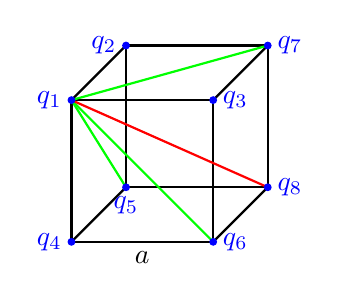
\begin{tikzpicture}[scale=.6]
                \draw[thick] (0,0,0) -- (0,3,0);
                \draw[thick] (0,0,0) -- (3,0,0);
                \draw[thick] (0,0,0) -- (0,0,3);
                \draw[thick] (0,0,3) -- (3,0,3);
                \draw[thick] (3,0,0) -- (3,0,3);
                \draw[thick] (0,0,3) -- (0,3,3);
                \draw[thick] (0,3,0) -- (3,3,0);
                \draw[thick] (3,3,0) -- (3,0,0);
                \draw[thick] (0,3,0) -- (0,3,3);
                \draw[thick] (3,3,3) -- (0,3,3);
                \draw[thick] (3,3,3) -- (3,0,3);
                \draw[thick] (3,3,3) -- (3,3,0);
                \draw[thick, green] (0,3,3) -- (3,0,3);
                \draw[thick, red] (0,3,3) -- (3,0,0);
                \draw[thick, green] (0,3,3) -- (0,0,0);
                \draw[thick, green] (0,3,3) -- (3,3,0);
                \filldraw[blue] (0,3,3) circle (2pt) node[anchor=east]{$q_1$};
                \filldraw[blue] (0,3,0) circle (2pt) node[anchor=east]{$q_2$};
                \filldraw[blue] (3,3,3) circle (2pt) node[anchor=west]{$q_3$};
                \filldraw[blue] (0,0,3) circle (2pt) node[anchor=east]{$q_4$};
                \filldraw[blue] (0,0,0) circle (2pt) node[anchor=north]{$q_5$};
                \filldraw[blue] (3,0,3) circle (2pt) node[anchor=west]{$q_6$};
                \filldraw[blue] (3,0,0) circle (2pt) node[anchor=west]{$q_8$};
                \filldraw[blue] (3,3,0) circle (2pt) node[anchor=west]{$q_7$};
                \node[anchor=north] at (1.5,0,3) {$a$};

            \end{tikzpicture}

            $F_e=q_1\vec{E_T}=q_1\Sigma\vec{E}=q_1(\mathrm{k}\frac{q_2}{a}\hat{r}+\mathrm{k}\frac{q_3}{a}\hat{r}+\mathrm{k}\frac{q_4}{a}\hat{r}+\mathrm{k}\frac{q_5}{a\sqrt[]{2}}\hat{r}+\mathrm{k}\frac{q_6}{a\sqrt[]{2}}\hat{r}+\mathrm{k}\frac{q_7}{a\sqrt[]{2}}\hat{r}+\mathrm{k}\frac{q_8}{a\sqrt[]{3}}\hat{r})$

            $F_e=\mathrm{k}\frac{q^2}{a}((0,0,-1)+(1,0,0)+(0,-1,0)+\frac{(0,-1, -1)+(1,-1,0)+(1,0,-1)}{\sqrt[]{2}}+\frac{(1,-1,-1)}{\sqrt[]{3}})$\\
            $=\mathrm{k}\frac{q^2}{a}((1,-1,-1)+(0,-\frac{1}{\sqrt[]{2}}, -\frac{1}{\sqrt[]{2}})+(\frac{1}{\sqrt[]{2}}, -\frac{1}{\sqrt[]{2}}, 0)+(\frac{1}{\sqrt[]{2}},0,-\frac{1}{\sqrt[]{2}}))+(\frac{1}{\sqrt[]{3}},-\frac{1}{\sqrt[]{3}},-\frac{1}{\sqrt[]{3}})$\\
            $=\mathrm{k}\frac{q^2}{a}((1,-1,-1)+(\frac{2}{\sqrt[]{2}},-\frac{2}{\sqrt[]{2}},-\frac{2}{\sqrt[]{2}})+(\frac{1}{\sqrt[]{3}},-\frac{1}{\sqrt[]{3}},-\frac{1}{\sqrt[]{3}}))$

            $F_e=\mathrm{k}\frac{q^2}{a}(1+\sqrt[]{2}+\frac{1}{\sqrt[]{3}},-1-\sqrt[]{2}-\frac{1}{\sqrt[]{3}}, -1-\sqrt[]{2}-\frac{1}{\sqrt[]{3}})$
        \end{center}

    \end{enumerate}

\end{document}
